\addcontentsline{toc}{chapter}{Appendix}
\label{ch:appendix}

\chapter{Initial Web Survey Results}
\label{ch:survey_results}

The following pages contain the results of the initial survey completed by both members of the Department of Computing and Electrical and Electronic Engineering.

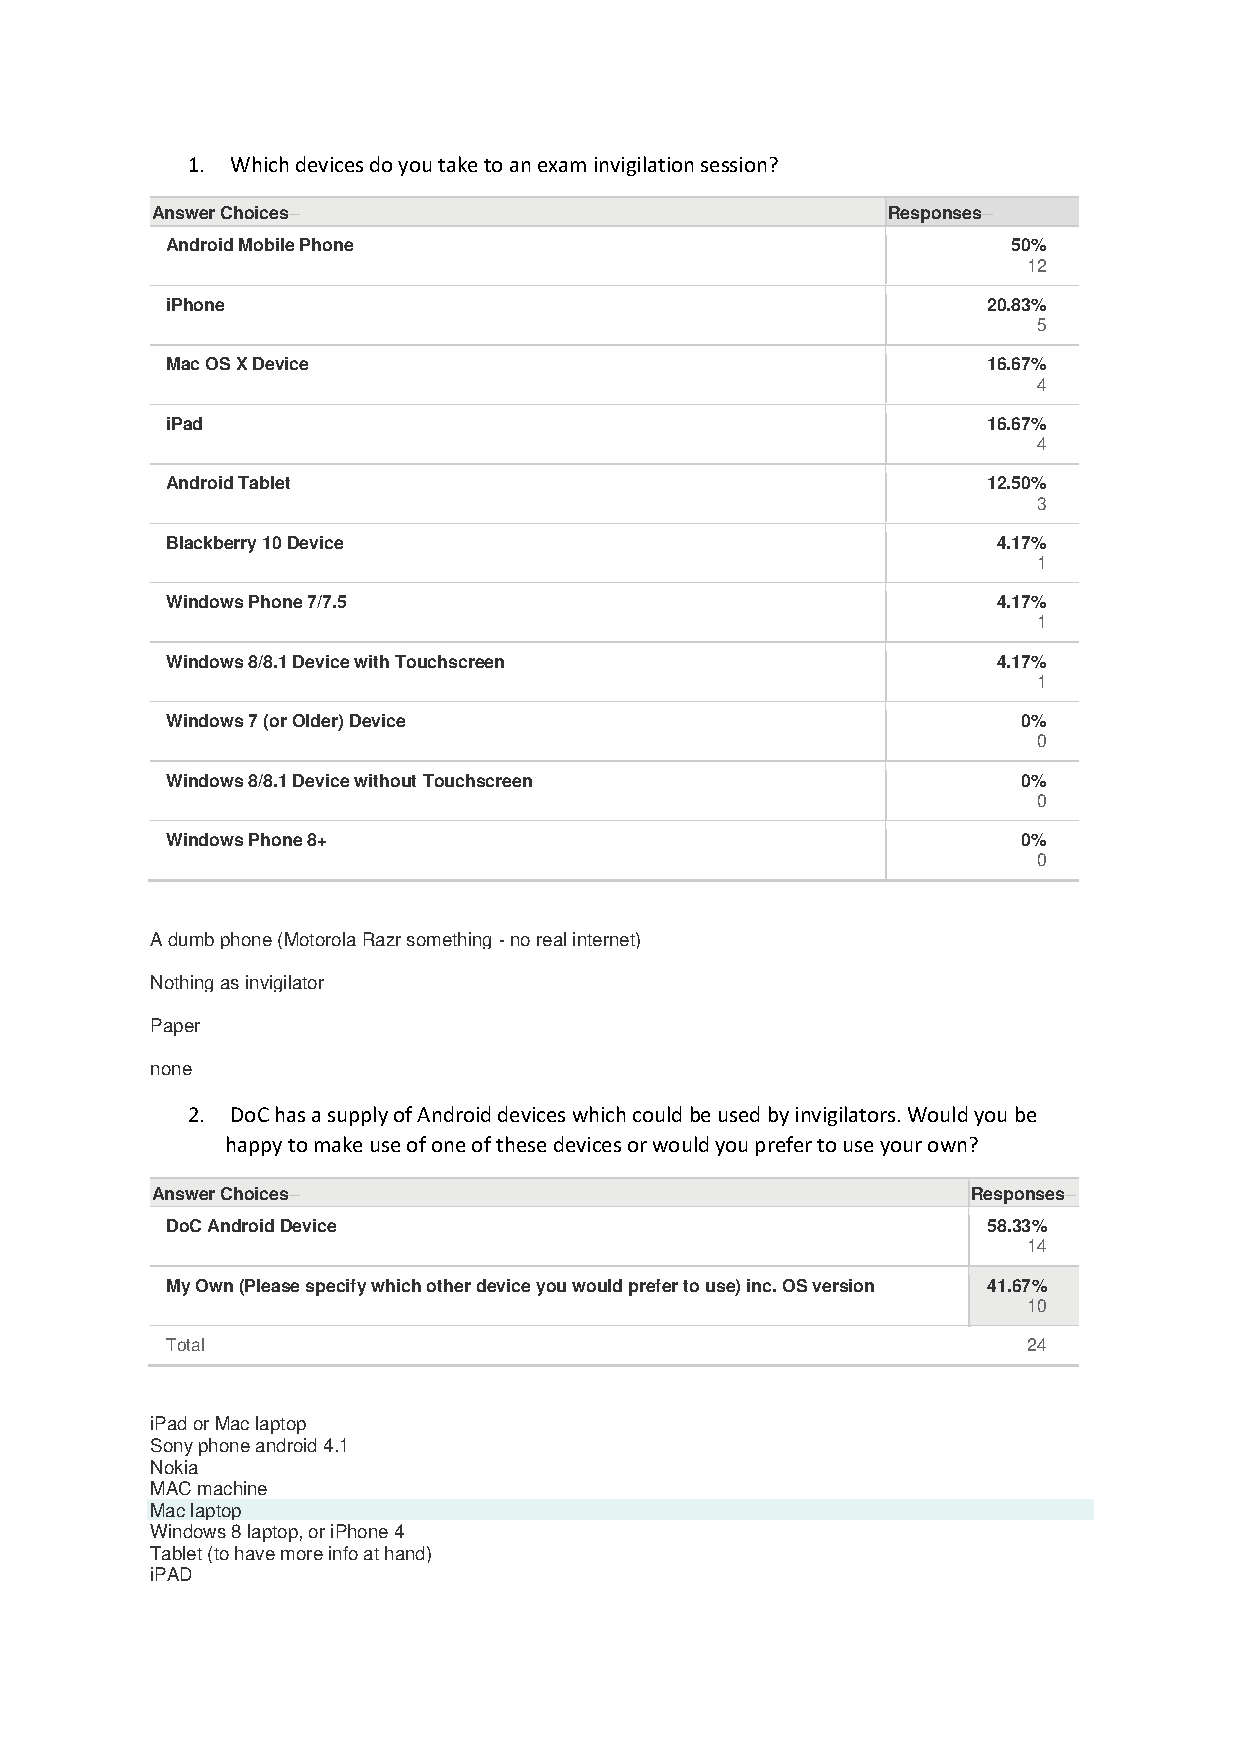
\includepdf[pages=-]{surveyresults/surveyResult.pdf}

\chapter{Evaluation Session Form}
\label{ch:exics_eval_doc}

The following pages contain the document used to complete the evaluation of ExICS with both members of the faculty and my peergroup to evaluate the usability and user experience of the ExICS client.

\includepdf[pages=-]{evaluation/peer_eval.pdf}

\chapter{User Guide}
\label{ch:user_guide}

There are three sections necessary to use ExICS.  The API Wrapper Server neccessary to convert the DoC provided exam and seating data into JSON, the ExICS back-end server which serves connecting clients and maintains system state, and the ExICS mobile client application.

\section{For System Administrators}

\subsection{ExICS Servers}

The ExICS servers run on the Node.JS platform.  It has been developed and tested using Node v0.10.28.

Once node.js is installed the following dependencies for the software must be installed using NPM, the node package manager.  The versions used during development and testing are shown after the @ symbol:

\begin{itemize}

\item activedirectory@0.2.2
\item mongodb@1.4.6
\item mongoose@3.8.12
\item querystring@0.2.0
\item request@2.34.0
\item ws@0.4.31

\end{itemize}

Because Node.JS is based on Javascript which is interpreted, the source files do not need compiling.

Assuming you are in the ``ExICS'' directory containing the server components, simple enter ``ExamDataCSVWrapper'' in a terminal and launch it with ``node examDataAPIServer.js''.

To run the ExICS server itself, from the ``ExICS'' root directory, enter the ``ExICSServer'' directory and run it with ``node ExICSServer.js''.

Before using the server there are some configurable options which can be adjusted.

\subsubsection{API Server}

In the requestHandlers.js file, csvURL on line 6 should be changed to point to the DoC API providing the exam information in tab separated format as described in section \ref{subsec:examData}.

The file seatingPlan.csv in the `Seating Plan' folder should be provided in the same form as described in section \ref{subs:seating_plan_info}.

examDataAPIServer.js can also be modified to change which ports both the HTTP and HTTPS servers listen on.  By default ports 8080 and 8443 are used respectively.  It is important to make a note of these port numbers for use in configuration of the ExICS server.

SSL Certificates should be generated and placed in a directory called ``ssl'' for use by the server. They should be named server.crt, server.csr, server.key and server.key.org.  The names of the certificates can be altered by modifying apiServer.js to alter the HTTPS server options provided lines 54 and 55.

\subsubsection{ExICS Server}

To use the ExICS server, first a file must be created with the other source files called AD\_CONFIG.js which contains the information shown in figure \ref{fig:ad_conf}.

\begin{figure}[!htbp]
\centering
\lstset{language=JavaScript}
\begin{lstlisting}[tabsize=2,breaklines=true]
var url = 'ldap://icadsldap.ic.ac.uk'; // URL of LDAP Server
var baseDN = 'dc=ic,dc=ac,dc=uk'; // Base Domain Name Being Checked
var username = '<username>@IC.AC.UK' // Username of Credentials to be Bound Against
var password = '<password>' // Password of Credentials to be Bound Against

exports.url = url;
exports.baseDN = baseDN;
exports.username = username;
exports.password = password;
\end{lstlisting}
\caption{AD\_CONFIG.js Contents Required for LDAP Authentication}
\label{fig:ad_conf}
\end{figure}

ExICSServer.js can be modified on line 26 to change the port to which the Websockets server listens.  By default it runs on port 8081.

In ExICSSystemData.js, line 423 must be modified to point to the hostname and port that the ExamData API server is running on.  If the SSL certificates for the Exam Data API server match its hostname and are signed by a trusted Certificate Authority, it is recommended to enable strict SSL on line 440.

Also in ExICSSystemData.js, if session start and end times are different than those used in development with 1.30pm used at the changeover point, they can be modified on lines 28-40.  If real exam data is being used, any references of ``var \textless name \textgreater = getMockTime()'' should have ``getMockTime()'' replaced with ``new Date()''.  Alternatively, if existing data is being used and you want to manually specify the date and time used whenever the system loads and refreshed, getMockTime() can be modified to manually specify the date and time being used.  By default getMockTime() provides a date of 2nd May 2013 at 9:27:35am.

\section{For Users}

The use of the ExICS client application has been designed to be as simple as possible.  Once the ExICS and Exam Data servers are running it can be used as follows.

The device being used must be connected to a network connection capable of accessing the host server, and the hostname and port of the ExICS server must be known if not already configured.

Open the ExICS app and click the menu symbol in the top right of the screen and select settings.  Click ``Hostname'' and make sure the hostname shown is that of the ExICS server.  Click OK and then click ``Port'' and make sure the port number shows matches that of the ExICS server.  Click ok and then press the ``Back'' button on the device to return to the Login Page.  A toast should be displayed saying settings updated.

Enter your college username and password, then click the Login button.  If you will be using the device again, you can check the ``Remember Credentials'' checkbox so you don't need to reenter them every time you open the app.

Click the ``Login'' button and the app will try and connect to the ExICS server.  If it is successful a room select dialog will appear asking you which room you want to be associated with.  If it does not appear, a toast will appear telling you why the connection attempt failed.  First check your credentials are correct, and if they definitely are, check with the system administrator that the ExICS server is definitely running.  If it is, check that the hostname of the server can be resolved by trying to open ``https://\textless hostname\textgreater :\textless port number\textgreater/examData/apidoc''.  If a message box asking for username and password appears, you can resolve the hostname.  Try and enter your college credentials.  If you are told you do not have permission, check with the college administrators to make you LDAP is working correctly.

Once a room is selected you will be taken to the main ExICS screen.  If the device is in landscape mode, the screen will be split in two with the ``Room Overview'' on the left and the ExICS log on the right.  If the device is in portrait, you will just see the ``Room Overview''.  The screen can be swiped left to reveal the ``ExICS log''.  Swipe right to get back to ``Room OverView''.

The app navigation drawer can be accessed by swiping right from the left edge of the screen, or by clicking the application icon in the top left.

Exams can be managed from the ``Overview'' section, seating plans viewed in the ``Seating Plan'' section, or the invigilation plan in the ``Invigilation Plan'' section.

In the overview, a red status light shows that an exam, or at least one exam in a room is currently stopped.  Green means that everything is OK and the exams are all running, amber means that an exam or at least one in a room is currently paused.

Messages can be sent by clicking the send message button at the bottom of the ``ExICS Log''.  Preset messages can be used to access predefined messages which can be sent, or custom can be used to type your own.  Messages can be sent to all users connected to the system, all users in a room, or to an individual by selecting the necessary recipient type.

When a message is received a dialog box will be displayed showing the message.  From this screen, you can dismiss the message, ignoring it, or send a reply selected from the dropdown menu which will be sent to the other person when reply is clicked.